%% The first command in your LaTeX source must be the \documentclass command.
\documentclass[acmtog, language=ngerman]{acmart}
\PassOptionsToPackage{english,ngerman}{babel}
%\usepackage[english,ngerman]{babel}
\usepackage[utf8]{inputenc} 

%% \BibTeX command to typeset BibTeX logo in the docs
\AtBeginDocument{%
  \providecommand\BibTeX{{%
    \normalfont B\kern-0.5em{\scshape i\kern-0.25em b}\kern-0.8em\TeX}}}
    
\copyrightyear{2024}
\acmYear{2024}
\citestyle{acmauthoryear}

\usepackage[figurename=Fig.]{caption}
\setcopyright{none}
\makeatletter
\renewcommand{\fnum@figure}{Abb. \thefigure}
\makeatother
\addto\captionsngerman{\renewcommand{\figurename}{Abb.}}
\settopmatter{printacmref=false} % Removes citation information below abstract
\renewcommand\footnotetextcopyrightpermission[1]{} % removes footnote with conference information in first column

%%
%% end of the preamble, start of the body of the document source.
\begin{document}
\selectlanguage{ngerman}

%%
%% The "title" command has an optional parameter,
%% allowing the author to define a "short title" to be used in page headers.
\title{Fähigkeiten und Vorgehen von Low-Code-Ansätzen}

%%
%% The "author" command and its associated commands are used to define
%% the authors and their affiliations.
%% Of note is the shared affiliation of the first two authors, and the
%% "authornote" and "authornotemark" commands
%% used to denote shared contribution to the research.
\author{Teo Förste}
\authornote{Alle Studierenden trugen zu gleichen Teilen zu dieser Arbeit bei.}
\author{Christin Göb}
\authornotemark[1]
\author{Chiara Schepke}
\authornotemark[1]
\affiliation{%
  \institution{\\
Hochschule für Technik, Wirtschaft und Kultur Leipzig}
  \streetaddress{Karl-Liebknecht-Str. 132}
  \city{Leipzig}
  \country{Deutschland}
  \postcode{04277}
}
%%
%% By default, the full list of authors will be used in the page
%% headers. Often, this list is too long, and will overlap
%% other information printed in the page headers. This command allows
%% the author to define a more concise list
%% of authors' names for this purpose.
\renewcommand{\shortauthors}{Förste, Göb, Schepke}

%%
%% The abstract is a short summary of the work to be presented in the
%% article.
\begin{abstract}
  %(Abstract-Länge ist typischerweise 15-25 Zeilen lang, in der PDF-Darstellung) 
  %A clear and well-documented \LaTeX\ document is presented as an article formatted for publication by ACM in a conference proceedings or journal publication. Based on the ``acmart'' document class, this article presents and explains many of the common variations, as well as many of the formatting elements an author may use in the preparation of the documentation of their work.
  Low-Code-Plattformen haben sich in den letzten Jahren als eine beliebte Alternative zur traditionellen Softwareentwicklung etabliert. \cite{studie_low_code} Durch die Möglichkeit, Anwendungen schnell und einfach zu entwickeln, ohne Erfahrungen auf dem Gebiet des Software Engineering zu benötigen, wurde eine neue Zielgruppe von Entwickelnden erschlossen: so genannte Citizen Developer. Die Anbieter von Low-Code-Plattformen bieten diesen ein komfortables Rundumpaket an Funktionalitäten und Dienstleistungen, damit sie sich voll und ganz auf die Umsetzung ihrer Idee konzentrieren können, ohne technisches Know-how zu benötigen. In dieser Arbeit wird untersucht, ob die Versprechen von Low-Code eingehalten werden können, welche Chancen und Risiken dieser neue Softwareentwicklungsansatz mit sich bringt und inwieweit er den Herausforderungen in größeren Entwicklungsteams gewachsen ist.
\end{abstract}

\maketitle

\section{Einleitung und Motivation}

\begin{figure}[h]
    \centering
    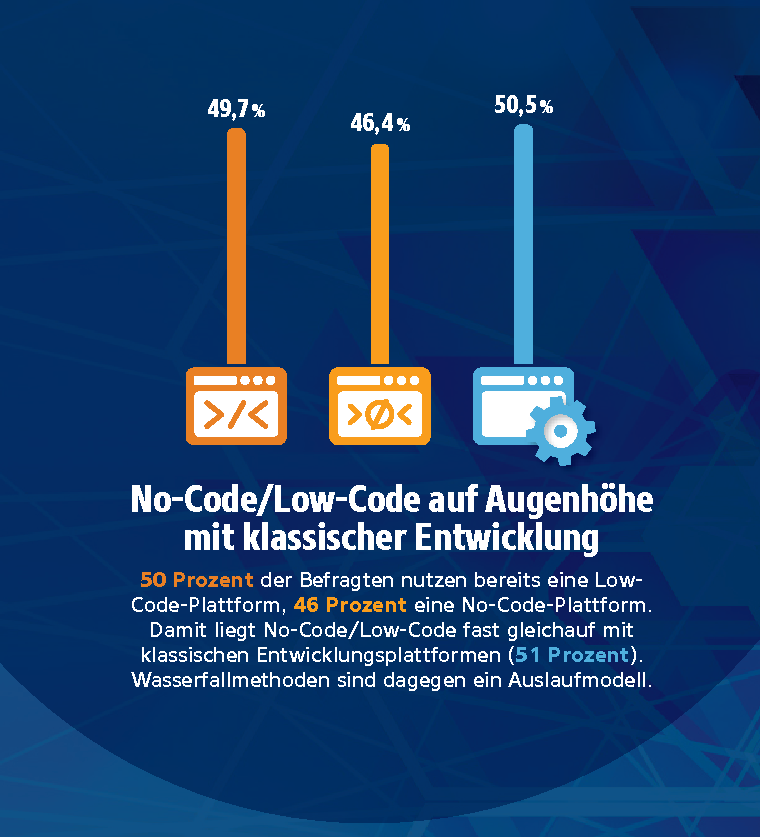
\includegraphics[width=1\linewidth]{images/studie-low-code-cropped.pdf}
    \caption{aus \cite{studie_low_code}}
    \label{fig:low_code_no_code}
\end{figure}
\subsection{Kontext}
Die mit großen Schritten voranschreitende Digitalisierung auf der einen und der Fachkräftemangel in der IT-Branche auf der anderen Seite begünstigen die Entwicklung und Verbreitung alternativer Methoden zur traditionellen Softwareentwicklung. \cite{flake_fachkraeftemangel_2023} Laut einer aktuellen Studie haben 50 Prozent aller Befragten bereits mit einer Low-Code-Plattform gearbeitet (s. Abb. \ref{fig:low_code_no_code}). Der weltweiten Marktgröße von Low-Code-Plattformen wird eine durchschnittliche jährliche Wachstumsrate von 27,8 Prozent vorhergesagt. Bis 2030 soll sie einen Gesamtwert von 148,5 Milliarden US-Dollar erreichen. \cite{straits_low_code_development_platform_market_2021} 

\subsection{Aufbau und Ziel der Arbeit}
In dieser Arbeit wird zunächst erklärt, was Low-Code-Plattformen sind, welche Low-Code-Ansätze schon länger bestehen und wie sie sich die Arbeit mit ihnen von der klassischen Softwareentwicklung unterscheidet. Anhand von ausgewählten Szenarien wird aufgezeigt, wie sich die Vor- und Nachteile gegenüber High-Code konkret äußern. Ferner sollen die Grenzen der Arbeit mit Low-Code beleuchtet werden. 

\section{Low-Code}
Dieses Kapitel führt den Begriff Low-Code auf sprachlicher sowie inhaltlicher Ebene ein. Anhand einiger ausgewählter Beispiele aus der Vergangenheit wird aufgezeigt, dass Ansätze aus dem Low-Code schon wesentlich länger Verwendung finden als der Begriff selbst.

\subsection{Terminologie}
Der Begriff setzt sich zusammen aus den Worten low (engl. niedrig) und code. Code meint dabei den Quellcode, während low sich auf die Menge an diesem in einem Softwareprojekt bezieht. "low [amount of] code" bedeutet also, dass nur eine möglichst geringe Menge an Quellcode geschrieben werden muss, um eine Software zu entwickeln. Zur Abgrenzung von der klassischen Softwareentwicklung, welche üblicherweise, und insbesondere bei umfangreichen Projekten, eine große Menge an Quellcode benötigt, ist für diese auch der Begriff High-Code geläufig. Eine weitere Variante dieser Namensgebung ist No-Code, welche eine extreme Form von Low-Code beschreibt. Bei No-Code wird im Gegensatz zu Low-Code vollständig auf von Hand geschriebenen Quellcode verzichtet. 

\subsection{Was ist Low-Code?} \label{sec:was_ist_low_code}
In seinem Beitrag "Low-code platform for automating business processes in manufacturing" listet Robert Waszkowski folgende Entwicklungsansätze auf, welche seiner Erkenntnis nach der Low-Code-Programmierung zu Grunde liegen:

\begin{itemize}
    \item Modellgetriebene Softwareentwicklung (Model Driven Development, MDD). Dieser stellt das Modell in den Mittelpunkt des Entwicklungsprozesses. Im Gegensatz zur unterstützenden Verwendung von Modellen im Rahmen eines Softwareentwicklungsprozesses, etwa zwecks Veranschaulichung, wird beim MDD der Quellcode semi- oder vollautomatisch aus dem erstellten Modell generiert. Dieser Ansatz findet sich in vielen Implementierungen des Low-Code-Prinzips.
    \item Schnelle Anwendungsentwicklung: Rapid Application Development, nachfolgend RAD abgekürzt, beschreibt eine Methode der Softwareentwicklung. Diese zielt speziell darauf ab, Anwendungen schnell und effizient zu erstellen. Der Fokus dabei liegt auf der schnellen Bereitstellung funktionsfähiger Software, wobei iterative Prozesse, die Beteiligung von Endbenutzer:innen und die Wiederverwendung von Softwarekomponenten im Vordergrund stehen.
Die Merkmale von RAD lassen sich wie folgt kategorisieren. Schnelle Iterationen, benutzerzentrierter Ansatz, Wiederverwendung von Komponenten, Protoyping, flexible Anpassung an Änderungen und visuelle Entwicklung. \cite{rapid_protoyping} RAD und das MVP \ref{sec:mvp} ergänzen sich in den meisten Punkten und können deshalb gut gemeinsam eingesetzt werden.
    \item Automatisierte Quellcodegenerierung: im Original Automatic Code Gerneration, meint die automatisierte Erstellung von Quellcode auf der Grundlage einer höheren Abstraktionsebene. Handelt es sich bei dieser um ein Modell, so kann dieses Verfahren als Ergänzung des modellgetriebenen Entwicklungsansatzes dienen.
    \item Visuelle Programmierung: Bei Visueller Programmierung, im Englischen Visual Programming, kurz VP,  handelt es sich um einen dem Low-Code-Prinzip ähnlichen Softwareentwicklungsansatz. Die Ähnlichkeit besteht im gemeinsamen Ziel, die Menge an manuell zu schreibendem Programmcode zu minimieren sowie dem visuellen Ansatz zum Erreichen dieses Ziels. Während grafische Elemente das Herzstück des visuellen Programmieransatzes darstellen, ist Low-Code hingegen nicht allein auf diese beschränkt.
\end{itemize}

Die Art und Weise, wie Quellcode, welcher von den Entwickelnden selbst zu schreiben ist, in der Softwarentwicklung konkret minimiert wird, unterscheidet sich von Plattform zu Plattform. Meist wird eine grafische Benutzerobfläche verwendet. Im Gegensatz hierzu wird in der High-Code Entwicklung meist eine Integrierte Entwicklunsumgebung, auf englisch integrated development  environment, kurz IDE, verwendet. 

Das Forschungsteam um Davide Di Ruscio hat in einem Expert Voice Paper für die IFAC untersucht, ob es sich bei Low-Code nicht einfach nur um eine neue, alternative Bezeichnung für den bereits bekannten modellgetriebenen Entwicklungsansatz handelt. Dabei kamen die Forschenden zu dem Ergebnis, dass sich die beiden Vorgehensweisen zwar in vielen Belangen ähneln, im Grunde aber dennoch zwei unterschiedliche Programmierkonzepte darstellen. \cite{low_code_vs_mdd}

\subsection{Low-Code im Kontext von Programmiersprachen}
Um den Low-Code-Entwicklungsansatz in der vielseitigen Landschaft der Programmiersprachen und -konzepte verorten und ihn in Relation zu dem Begriff der Fourth Generation Language, kurz 4GL, setzen zu können, sei die Entwicklung von Programmiersprachen in der üblichen Anordnung nach Generationen im Folgenden kurz umrissen.

\begin{enumerate}
    \item Als Programmmiersprachen der ersten Generation werden von Maschinen lesbare Binärcodes bezeichnet. Dabei handelt es sich um einen Satz prozessorspezifischer Befehle, welche nicht vom Menschen gelesen werden können. Gleichzeitig ist diese Sprache ihrer zugehörigen Hardware am allernächsten.
    \item Die nächste Generation bilden die Assemblersprachen, welche den binär codierten Befehlssatz einer Maschinensprache in eine vom Menschen lesbare Syntax übersetzen. Dabei bleiben die hardwarespezifischen Eigenschaften der ersten Generation bestehen, sodass jeder Prozessor eine eigene, seinem Befehlssatz zugehörige Assemblersprache besitzt.
    \item Programmiersprachen der dritten Generation sind klassische Hochsprachen wie Java, C++ oder Python, die es den Entwickelnden erlauben, komplexen, prozessorübergreifenden Code zu schreiben, welcher anschließend zwecks Ausführung von einem Compiler oder Interpreter in den passenden Maschinencode des jeweiligen Zielsystems übersetzt wird.
    \item Der Begriff der Fourth Generation Language ist bisher nicht eindeutig definiert und wird hauptsächlich \glqq als Marketinginstrument verwendet, um ein neues Programm oder eine weitere Sprache durchzusetzen\grqq. \cite{handbuch_programmiersprachen} Grundsätzlich handelt es sich dabei um alle Entwicklungsansätze, welche versuchen, die Funktionalität von klassischen, prozeduralen Sprachen mit weniger Code umzusetzen, indem das Abstraktionsniveau noch weiter erhöht wird. Als konkretes Beispiel für 4GL nennen Henning und Vogelsang in ihrem Handbuch Programmiersprachen die Abfragesprache SQL (Structured Query Language), aber auch allgemeine deskriptive Sprachen und Skriptsprachen.
\end{enumerate}

Basierend auf diesem Modell verortet Waszkowski den Low-Code-Entwicklungsansatz auf einer noch höheren Abstraktionsebene und bezeichnet ihn als Weiterentwicklung von Programmiersprachen der vierten Generation im Zusammenspiel mit dem Konzept des Rapid Application Development (RAD). \cite{waszkowski_2019}

\subsection{Low-Code-Ansätze in der Vergangenheit}
Erstmals eingeführt im Jahr 2011, beschreibt der Begriff Low-Code ein modernes sowie, basierend auf den Ergebnissen der Low-Code/No-Code-Studie \cite{studie_low_code}, durchaus zukunftsfähiges Entwicklungskonzept. Nichtsdestotrotz offenbart ein Blick in die Geschichte, dass einige Ansätze aus dem Low-Code bereits seit Jahrzehnten zur Anwendung kommen und den Entwickelnden ihre Arbeit erleichtern.

Bei folgenden Beispielen handelt es sich um Softwareentwicklungstools aus den 80er- und 90er-Jahren, welche eines oder mehrere Merkmale aufweisen, die nach heutiger Definition dem Low-Code-Entwicklungsansatz inhärent sind. Zu beachten ist, dass es sich dabei ausdrücklich nicht um Low-Code-Plattformen handelt.

Die folgende Auswahl bezieht sich größtenteils auf einen Beitrag von Michael Bünning zur Microsoft Power Plattform. \cite{microsoft_power_platform}

\begin{itemize}
    \item Mit der Einführung des Apple Macintosh im Jahr 1984 eroberte erstmals ein Personal Computer mit grafischer Benutzeroberfläche den Markt, was für die damalige Zeit eine revolutionäre Neuerung darstellte. Eines der ersten Programme, welches sich diese zunutze machte, war der \textbf{File Maker}, ein Datenbankmanagementsystem, kurz DBMS, von Nashoba Systems aus dem Jahr 1985. Es ermöglichte den Nutzenden, Datenbanken bequem mittels einer formularbasierten GUI zu erzeugen und zu verwalten, anstatt die entsprechenden SQL-Queries manuell verfassen zu müssen. \cite{filemaker_history}
    \item Im Jahr 1989 erschien mit \textbf{Lotus Notes} ein Groupwareprogramm mit E-Mail-Integration. Dieses bot von Beginn an eine Formularsprache zur einfacherern Programmierung von Notes. Seit Version 5 (1999) zählt zum Produktumfang auch eine integrierte Entwicklungsumgebung namens \textbf{Domino Designer}, welche speziell auf die schnelle Anwendungsentwicklung (RAD) ausgerichtet ist. \cite{history_of_notes_and_domino}
    \item Zu den wohl bekanntesten Beispielen in dieser Aufzählung zählt \textbf{Visual Basic} von Microsoft (1991), eine integrierte Entwicklungsumgebung für die Erstellung von Desktop-Anwendungen für das Betriebssystem Windows. Der visuelle Editor mit Drag-and-Drop-Funktionalität, welcher der Software ihren Namen gibt, ist  ausschlaggebend für die Klassifizierung als Low-Code-Vorgänger. Jeff Goldberg geht sogar so weit, moderne Low-Code/No-Code-Plattformen sinngemäß als das Visual Basic unserer Zeit zu bezeichnen: \glqq It’s hard to see the modern Low-Code/No-Code platforms as anything other than Visual Basic for the internet and mobile age\grqq. \cite{goldberg_visual_basic}
    \item PowerSoft veröffentlichte im Jahr 1992 eine Visual Basic ähnliche Entwicklungsumgebung namens \textbf{PowerBuilder}. Zu den aus Visual Basic bekannten Low-Code-Ansätzen kam beim PowerBuilder automatisch generierter SQL-Code mit der DataWindow-Klasse.
    \item Ebenfalls im Jahr 1992 brachte Microsoft mit \textbf{Access} sein eigenes Datanbankmanagementsystem für das Betriebssystem Windows heraus. Michael Aldridge, Programmmanager von Access, bezeichnete seine Software in einem Vortrag auf der Ignite-Konferenz von 2021 als einen der Begründer der Entwicklung von Low-Code/No-Code-Lösungen, bevor es dafür überhaupt einen Begriff gab: \glqq It's also one of the originators of the low-code/no-code solution development before it was even called that.\grqq \cite{aldridge} In einem Bericht über besagte Konferenz kritisiert Daniel Pineault diese Behauptung und stellt die Eigenschaften von Access der Definition einer Low-Code-Plattform gegenüber. Obgleich er zu dem Schluss kommt, dass es sich bei Microsoft Access im Großen und Ganzen um eine High-Code-Plattform handelt (\glqq [...] as a whole, Access is a high-code platform.\grqq) \cite{pineault}, so nennt er dennoch einige Aspekte an dieser Software, welche seiner Aussage nach \glqq most definitely low-code/no-code\grqq, also eindeutig dem Low-Code-Ansatz zuzuordnen sind:
    \begin{itemize}
        \item der visuelle Tabellendesigner
        \item Query by Example, eine leicht verständliche Abfragesprache, die es Nutzenden ohne SQL-Kenntnisse erlaubt, Datenbankabfragen anhand von Beispieldaten zu verfassen.
        \item die Erstellung von Formularen oder Berichten mithilfe eines grafischen Wizards
        \item der Multifunktionsleistendesigner (Ribbon Customizer)
    \end{itemize}
    \item Auch das GUI-Framework \textbf{Qt}, welches 1995 veröffentlicht wurde, bietet einige Low-Code-Funktionalitäten. Insbesondere die vielen dazugehörigen Module sorgen dafür, dass Apps zum Teil ohne selbstgeschriebenen Code entwickelt werden können. \cite{piccolino}
\end{itemize}

Aus den genannten Beispielen lässt sich folgende Liste an Merkmalen und Funktionalitäten zusammentragen, welche heute als essenzielle Bestandteile von Low-Code-Plattformen angesehen werden. Dazu zählen auch die vier Ansätze nach Robert Waszkowski. (vgl. Kap. \ref{sec:was_ist_low_code})

\begin{itemize}
    \item Abstraktion
    \item Visualisierung
    \item Codegenerierung
    \item Integration eigener Skripte
    \item Schnelle Anwendungsentwicklung
    \item Bereitstellung vorgefertigter Funktionalitäten
\end{itemize}

Insbesondere der letzte Stichpunkt ist für das folgende Kapitel von Bedeutung.

\subsection{Eine neue Zielgruppe} \label{sec:citizen_developer}
Die modellgetriebene Natur des Low-Code-Entwicklungsansatzes und der Verzicht auf die Notwendigkeit von handgeschriebenem Code ermöglichen es auch informationstechnischen Laien ohne Programmierkenntnisse, Software zu entwickeln. Für diese neue Art der Softwareentwickelnden hat sich der Begriff \textbf{Citizen Developer} etabliert. In ihrer Studie \textit{The Rise of the Citizen Developer} beschreiben Marten Oltrogge et al. Citizen Developer als \glqq developers with little or no software engineering background\grqq, also Entwickelnde mit wenig oder gar keiner Erfahrung im Software Engineering. \cite{oltrogge_2018}

Die Anbieter von Low-Code Entwicklungsumgebungen unterstützen die Erschließung dieser neuen Zielgruppe durch die Bereitstellung weiterer Werkzeuge und Dienstleistungen. \cite{low_code_vs_mdd}

Die Betreiber der Low-Code-Plattform FlutterFlow werben auf ihrer Website unter anderem mit folgenden Funktionen: \cite{flutterflow_features}

\begin{itemize}
    \item Versionskontrolle durch Branching
    \item Erstellen von Tests für die einzelnen Komponenten
    \item Bildschirmaufnahmen (z. B. zwecks Marketing)
    \item Cloud-Funktionalitäten mit Firebase
\end{itemize}

Auch Arbeitsschritte, die über den eigentlichen Entwicklungsprozess hinausgehen, wie etwa die Veröffentlichung des fertigen Produkts auf verschiedenen Plattformen, werden als Dienstleistung angeboten.\cite{flutterflow_deployment} Mit einem solchen Rundumpaket können sich die Citizen Developer voll und ganz auf den Aufbau, die Struktur, das Design und die Funktionalität ihrer Software konzentrieren. Welche Nachteile dieses Entwicklungskonzept gegebenenfalls mit sich bringen kann, wird im weiteren Verlauf dieser Arbeit thematisiert.

\section{Vorgehensweisen in Softwareprojekten}

Nachdem die grundlegenden Konzepte von Low-Code im vorigen Abschnitt behandelt wurden, werden im folgenden Abschnitt verschiedene Szenarien beschrieben, an denen dargestellt wird, wie ein Softwareunternehmen Low-Code einsetzen kann. Hierbei werden gängige Methodiken der Softwareentwicklung benannt und die Vorteile beziehungsweise Nachteile, die sich durch die Verwendung von Low-Code-Ansätzen ergeben, aufgezeigt.
Begonnen wird mit einer Auflistung von Problemen und erörtert, welche Probleme speziell in großen Softwareunternehmen auftreten.

\subsection{Low-Code in großen Softwareunternehmen }

Gängige Problematiken, die bei der Entwicklung von Software unabhängig von der Größe des Teams auftreten können, sind: 
\begin{itemize}
\item Wartung von Bestandscode

Während der Laufzeit müssen Ressourcen aufgebracht werden, um Software lauffähig zu halten. Je länger die Laufzeit, desto höher das Risiko, dass der Quellcode veraltet und eventuelle Sicherheitslücken auftreten. 

Das Erweitern von Bestandscode durch neue Funktionalitäten birgt ebenfalls verschiedene Hürden. Eventuell existiert keine ausreichende Dokumentation, durch mangelnden Überblick seitens der Entwickler können Änderungen neue Probleme erzeugen, statt positive Effekte zu erzielen.

\item Dependency Management

Es muss beachtet werden, dass Abhängigkeiten regelmäßig aktualisiert werden müssen, um gewährleisten zu können, dass keine Kompatibilitätsprobleme und  Sicherheitslücken auftreten können.

\item Kompatibilitätsprobleme

Wird nicht auf Kompatibilität geachtet, kann es schon während der Entwicklung eines Projektes zu Problemen mit unterschiedlichen Plattformen, Browsern und Komponenten von Drittanbietern kommen. 

\item Testautomatisierungs- und Testumgebungsmanagement

Tests sollten in jeder Stufe der Entwicklung genutzt werden, um die Qualität des Produktes und des Codes zu prüfen.

\item Scalability

Software muss Veränderungen in der Menge der Benutzeranfragen und Data-Loads standhalten können.

\item Sicherheitsaspekte

Mögliche Sicherheitslücken müssen erkannt und geschlossen werden.

\item Gesetzliche Regulationen

Neue gesetzliche Vorschriften wie die DSGVO müssen in der Softwareentwicklung berücksichtigt und umgesetzt werden.

\item Fachkräftemangel

Der Mangel an ausgebildetem Fachpersonal muss in der Planung von Softwareprojekten berücksichtigt werden.

\item Wissensweitergabe \& Onboarding

Wenn neue Personen Teil eines Teams werden, sollte Wissen, welches essentiell für die neue Rolle der Person ist, und generelles Wissen über den neuen Arbeitsplatz vermittelt werden. Diese Wissensweitergabe kann sich in einigen Fällen schwierig gestalten. Wenn beispielsweise eine Person die sich im Rahmen ihrer Aufgaben, sehr spezifisches Wissen angeeignet und dieses nicht Dokumentiert hat, die Firma verlässt bevor eine neue Person eingestellt werden kann, ist das Wissen eventuell nicht mehr abrufbar.

\item Kommunikation

Je größer ein Projekt, ein Entwicklungsteam oder ein Unternehmen ist, desto mehr Personen müssen miteinander kommunizieren. Hierbei können mehrere Probleme auftreten.
Wenn ein Unternehmen viele Projekte umsetzt, liegen diesen oft unterschiedliche Anforderungen zugrunde. Wenn nun neue Standards eingeführt werden sollen, können diese in einem der Projekte sehr leicht, im nächsten nur sehr schwer umsetzbar sein. 
Teilweise müssen unternehmensweite Veränderungen von Coding-Standards koordiniert und durch Überprüfung gewährleistet werden, dass diese auch beibehalten werden. Teams können untereinander konkurrieren und Anforderungen völlig unterschiedlich interpretieren und umsetzen. Manche Projekte versuchen aufgrund ihrer Anforderungen sogar, gegenteilige Ergebnisse zu erzielen. 
\end{itemize}

Low-Code-Plattformen bieten für alle im vorigen Abschnitt genannten Probleme Lösungen, die auf bereits etablierten Konzepten basieren. Grundlegende Überlegungen, zum Beispiel die Frage, wie die Wartbarkeit des Projektes gewährleistet werden kann, werden den Nutzenden abgenommen. Low-Code-Plattformen bieten vollständig implementierte Mechanismen, die die entsprechenden Funktionalitäten abdecken. Eventuell wird eine Individualisierung durch eine Auswahl an Einstellungsänderungen geboten, um verschiedene Fälle abzudecken.
Wiederverwendbarkeit ist ein weiteres wichtiges Konzept von Low-Code-Plattformen.
Wenn innerhalb der Plattform individuelle Konfigurationen vorgenommen werden, sind diese zentralisiert verfügbar und können leicht wiederverwendet werden. 
Viele Plattformen bieten auch in der Implementierung von Quellcode verschiedene vorgefertigte Komponenten, die beliebig oft wiederverwendet werden können. Eine beschränkte Auswahl an Komponenten bietet den Plattformen die Möglichkeit, mehr Fokus auf die Qualität der einzigen Komponenten zu legen und testbare und vollständige Funktionalitäten zur Verfügung zu stellen.
Im Abschnitt \href{}{\ref{sec:UI}} wird beschrieben, wie Änderungen des Brand-Designs zentralisiert in einer Low-Code-Plattform umgesetzt werden können. Diese Vorgehensweise lässt sich auf sämtliche Änderungen innerhalb eines Teams mit mehreren Projekten übertragen. Anstatt Änderungen einzeln im Quellcode von verschiedenen Projekten aufwendig vorzunehmen, können sie zentralisiert innerhalb des Low-Code-Systems umgesetzt werden.

\subsection{Aktuelle Nutzung von Low-Code in Unternehmen}\label{sec:Aktuelle_Nutzung}

In einer Studie aus München aus 2023 wurden 386 Teilnehmende zu verschiedenen Dingen bezüglich der Nutzung von Low-Code in unterschiedlich großen Unternehmen befragt. \cite{studie_low_code}  Diese Studie wurde in verschiedenen Branchen mit der Hilfe von insgesamt 386 Interviews durchgeführt. 
In einer Befragung von 386 Teilnehmenden dieser Studie wird die Verwendung von Low-Code-Plattformen im Hinblick auf die Art und Weise der Entwicklung in den Unternehmen mit klassischen Softwareentwicklungsplattformen, No-Code-Plattformen, agilen Methoden wie etwa SCRUM oder Kanban sowie dem klassischen Wasserfallmodell auf eine Stufe gestellt und miteinander verglichen.
In den Unternehmen, die Software und Apps selbst entwickeln, wurde bei Mehrfachnennung zu 50,5 Prozent auf die klassischen Softwareentwicklungsplattformen zurückgegriffen und bereits zu 48,7 beziehungsweise 46,4 Prozent \cite{studie_low_code} zu Low-Code- beziehungsweise No-Code-Plattformen. Das bedeutet, dass die Hälfte der Unternehmen eine Low-Code-Plattform nutzen.
Die Unterschiede zwischen kleinen, mittelständischen und großen Unternehmen soll die folgende Abbildung \ref{fig:lowcode_nutzer} verdeutlichen.
\begin{figure} [h]
    \centering
    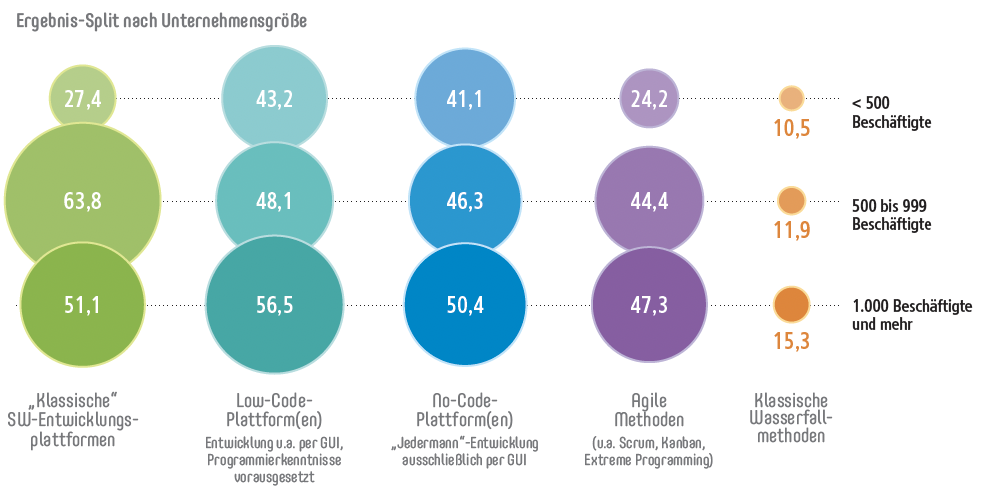
\includegraphics[width=1\linewidth]{images/studie_lowcodenutzer.png}
    \caption{Softwareentwicklungs-Methoden Ergebnisse \cite{studie_low_code}}
    \label{fig:lowcode_nutzer}
\end{figure}
Hierbei war die Frage, auf welche Art und Weise das Unternehmen jeweils Software entwickelt. Bei der Befragung haben 386 Teilnehmende mitgewirkt. Die Abbildung \ref{fig:lowcode_nutzer} verdeutlicht, dass in eher kleinen Unternehmen, welche hier mit 500 und weniger Beschäftigten kategorisiert werden, für die Softwareentwicklung am ehesten Low-Code und No-Code-Plattformen verwendet werden.
In mittelständischen Unternehmen (500 bis 999 Beschäftigte) überwiege die klassische Herangehensweise an die Softwareentwicklung. 
In großen Unternehmen, welche in dieser Studie jene sind, die 1000 oder mehr Beschäftigte angestellt haben, ist die Verwendung der Plattformen auf die vier Kategorien weitestgehend gleichverteilt.
\\

In einer weiteren Befragung, bei der 295 Teilnehmende mitgewirkt haben, wird deutlich, dass fast alle Unternehmen bei Low-Code auf Spezialplattformen setzen und 94 Prozent \cite{studie_low_code} der Befragten mindestens zwei No-Code- oder Low-Code-Plattformen in Kombination nutzen.
\\

Von 295 Befragten stimmen 68,8 Prozent \cite{studie_low_code} zu, dass die Corona-Pandemie, der Ukraine-Krieg, die Inflation und ähnlich gewichtige Ereignisse und Entwicklungen in den letzten Jahren Einfluss auf den Einsatz von Low- und No-Code-Lösungen haben.
Die Gründe dieser Einflüsse und der vermehrten Verwendung von Low-Code-Ansätzen werden in der nachfolgenden Abbildung \ref{fig:lowcode_gruende} aus der Studie von \cite{studie_low_code} deutlich gemacht.
\begin{figure}[h]
    \centering
    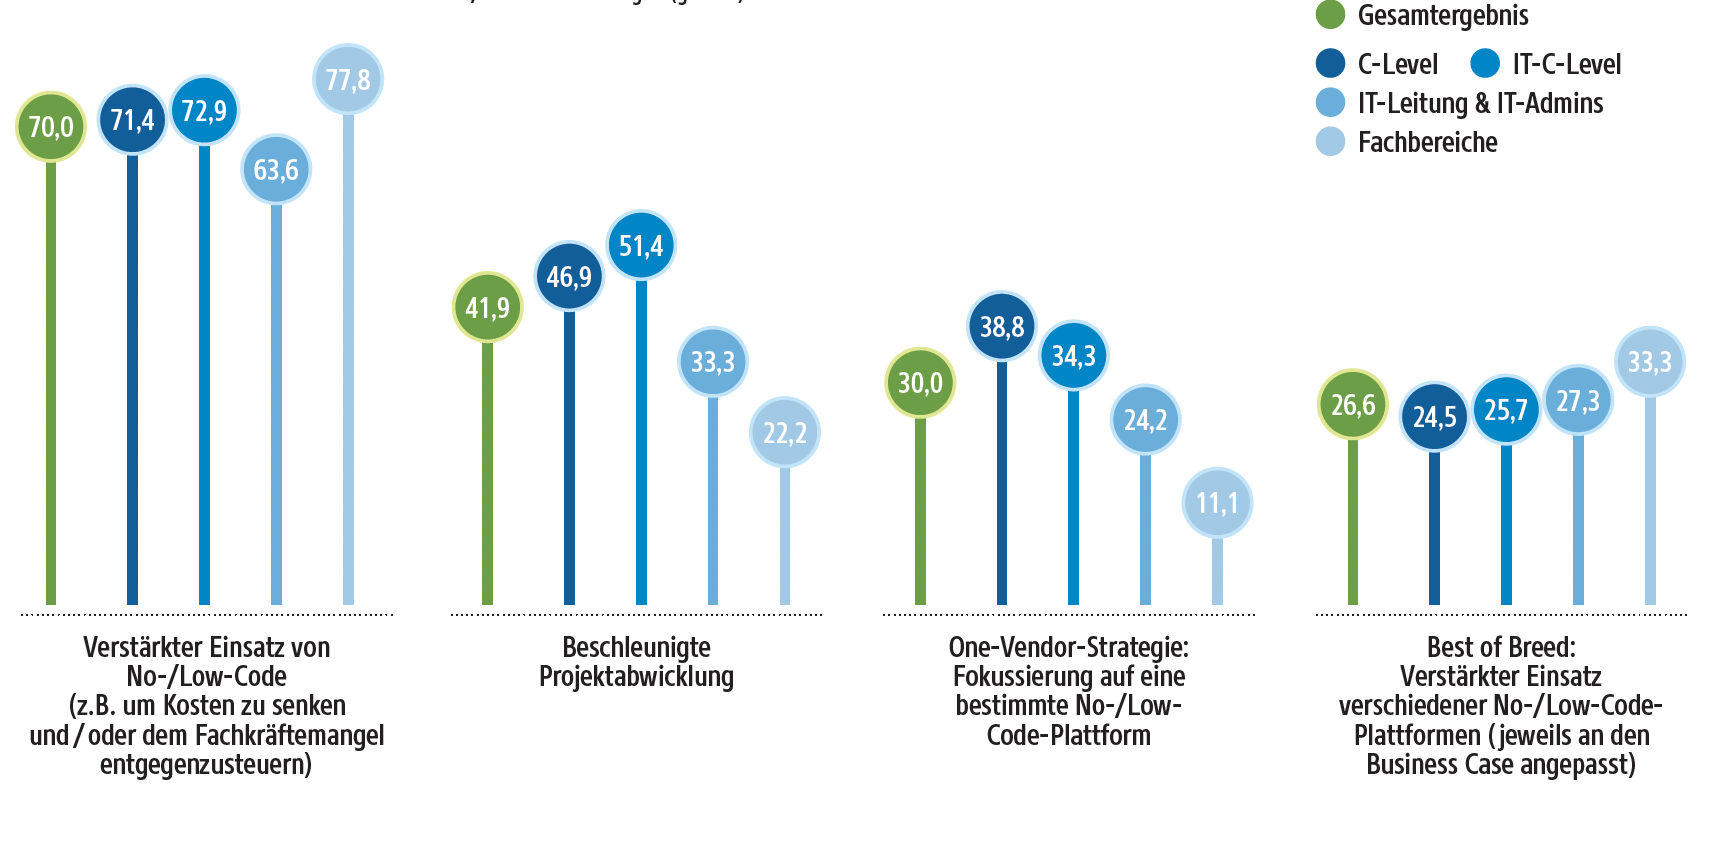
\includegraphics[width=1\linewidth]{images/studie_gruende.png}
    \caption{Gründe für die Nutzung von Low-Code nach Krisen \cite{studie_low_code}}
    \label{fig:lowcode_gruende}
\end{figure}
\newline
Hieraus kann man deutlich erkennen, dass der Kostenfaktor in vielen Unternehmen der wichtigste Aspekt ist, weshalb Low-Code- und No-Code-Plattformen in Betracht gezogen werden. Dabei ist wichtig zu nennen, dass dies eher bei den jeweiligen Fachbereichen der Fall ist.

\subsection{Minimum Viable Product} \label{sec:mvp}
Ein zentraler Aspekt der agilen Softwareentwicklungsmethodik ist das Minimum Viable Product, nachfolgend als MVP abgekürzt. Es ist eine bestimmte Art und Weise, wie ein Softwareentwicklungsprojekt organisiert werden kann.
Das Grundprinzip des MVP ist es, früher Zufriedenheit beim Kunden zu schaffen und kontinuierliche Optimierung umzusetzen. In die deutsche Sprache übersetzt bedeutet MVP, dass es darum geht, die minimale mögliche Umsetzung eines Softwareprojekts zu finden.

\begin{figure}[h]
    \centering
    
\includegraphics[width=1\linewidth]{images/mvp_grafik.jpg}
    \caption{Agiles Vorgehen: MVP-Gedanke \cite{mvp_definition}}
    \label{fig:mvp_figure}
\end{figure}
Die Abbildung Nummer \ref{fig:mvp_figure} von Marty True \cite{mvp_definition} soll zeigen, dass es insgesamt bei der agilen Methodik darum geht, ständig an der Grundidee weiterzuarbeiten. Das geplante beziehungsweise entwickelte Produkt soll immer weiter optimiert werden.
Dabei ist wichtig, dass das MVP immer ein Produkt ist, welches von Grund auf funktioniert. Es existiert eine sehr hohe Wahrscheinlichkeit, dass dabei einige Funktionen des Produkts reduziert werden müssen, um dies zu gewährleisten.
Im Fokus dieser Methodik steht also, sich erst einmal ausschließlich auf das zu fokussieren, was wirklich benötigt wird. Das minimale Produkt zu finden, was die grundlegenden Bedürfnisse stillt, ist das Ziel dieser Methodik.
Bei dieser Herangehensweise geht es nicht darum, den Kunden beziehungsweise die Kundin glücklich zu machen, sondern dass man im Prozess lernt, welche Anforderungen an das Produkt gestellt werden.

Das Prinzip des MVP beschränkt sich nicht auf die erste Iteration und den ersten Prototypen. Es kann immer weiter optimiert werden und würde sich dann beispielsweise MVP-\textit{X} und dann MVP-\textit{X+1} nennen. Es muss immer sichergestellt werden, dass das jeweilige MVP einsatzfähig ist.

\subsection{Low-Code MVPs}

Firma A möchte, dass für ihre neue Produktlinie ein Online-Shop entwickelt wird. Da die Produkte schon produziert werden, möchten die Stakeholder, dass der Shop schnellstmöglich produktiv genutzt werden kann.

Das Entwicklungsteam hat bisher ausschließlich native Apps mit Hilfe des Frameworks Flutter entwickelt. Der Webshop verkörpert die erste Web-App, die das Team entwickelt. Um Zeit zu sparen, wird die Entscheidung getroffen, FlutterFlow zu verwenden. In wenigen Arbeitsstunden soll ein MVP (Minimum Viable Product) entwickelt werden, damit so schnell wie möglich ein funktionaler Webshop angeboten werden kann.

In High-Code-Projekten ist es wichtig, sich zu Beginn eines neuen Projektes, insbesondere, wenn neue Technologien eingesetzt werden, mehrere Fragen zu beantworten: 

\begin{itemize}
    \item Wie ist das neue Projekt in die bereits bestehende Systemlandschaft integrierbar? 
    \item Welche Sicherheitslücken müssen beachtet und geschlossen werden?
    \item Wie lässt sich die Wartbarkeit des Produkts garantieren? 
    \item Wie kann der Quellcode zu einem späteren Zeitpunkt erweitert werden? 
    \item Wie setzt man die Anbindung vom Frontend zum Backend um? 
    \item Welche Schnittstellen müssen erweitert, angepasst oder neu entwickelt werden? 
\end{itemize}

Low-Code-Anbieter scheinen Lösungen für diese Themen zu bieten, jedoch kann dies zu einer starken Abhängigkeit führen. Unternehmen sollten abschätzen, wie aufwendig eine Migration in ein anderes System im Falle einer Auflösung des Low-Code-Anbieters ist. 

Nachdem Firma A die geforderten MVPs umgesetzt hat, ergibt sich für das Entwicklungsteam die Möglichkeit, die Entwicklung auf unterschiedliche Arten fortzuführen. Für den Fall, dass Funktionalitäten durch Low-Code nicht wie gewünscht umsetzbar sind, bieten Low-Code-Anbieter die Möglichkeit, einzelne Funktionalitäten mithilfe von High-Code-Fragmenten zu entwickeln. Falls dies nicht ausreicht, bietet FlutterFlow einen Export des von der Plattform generierten Flutter-Quellcodes an. Erfahrene Flutter-Entwickler:innen können diesen Code wie herkömmlichen High-Code behandeln.

Im Falle des beschriebenen Szenarios besteht eine Abhängigkeit nur über die Zeit, in der die ersten Versionen und Erweiterungen des MVP entwickelt werden. Da die Nutzung des Low-Code-Anbieters also auf einen beschränkten Zeitraum innerhalb der Projektlaufzeit genutzt wird, sollten keine Probleme durch eine Abhängigkeit vom Low-Code-Anbieter auftreten.

\subsection{Low-Code-Prototypen}

Das UX-Team von Firma A möchte für eine neue App Prototypen entwickeln, um damit User-Tests durchzuführen. In vergangenen Projekten wurden im Team mit gängigen UI \& UX Tools Prototypen entwickelt, welche für User-Tests genutzt wurden. Nach deren Abnahme wurden diese an die Entwicklungsabteilung gegeben, um anschließend mit High-Code umgesetzt zu werden. Für die neuen Prototypen entscheidet sich das Team jedoch dafür, die Prototypen direkt vom UX-Team als Low-Code MVPs umzusetzen, um High-Code-Entwicklungskapazitäten zu sparen. 

Des Weiteren bietet die Verwendung von Low-Code-Technologien die Möglichkeit, Prototypen schnell mit Funktionalitäten auszustatten oder direkt MVPs von UX/UI-Designern als Citizen Developer umsetzen zu lassen, auch wenn diese keine bisherigen Erfahrungen mit Programmieren haben (s. Kap. \ref{sec:citizen_developer}) 
Es wird hierbei davon ausgegangen, dass Citizen Developer bessere Lösungen für ihre Probleme entwickeln können als herkömmliche, vermutlich fachfremde Entwickelnde. Hierbei ist zu berücksichtigen, dass Low-Code-Plattformen keinen Ersatz für das Durchdenken von Problemen darstellen.
Man kann jedoch davon ausgehen, dass Verständnisprobleme, die üblicherweise bei der Weitergabe von Anforderungen auftreten, wegfallen. Dementsprechend kann Low-Code das Erstellen von Prototypen stark vereinfachen. \cite{Strengths_and_Weaknesses_of_Low-Code/No-Code_Tools_2022}


\subsection{Low-Code und SCRUM}

Firma A geht in ihrem High-Code-Entwicklungsprozess nach der agilen SCRUM-Methode vor. Sogenannte Sprints werden für einen Zeitraum von zwei Wochen geplant. Innerhalb dieser soll eine festgelegte Auswahl von Features vollständig oder teilweise umgesetzt werden.

Um Low-Code in seinen Entwicklungsprozess zu integrieren, entscheidet das Entwicklungsteam, während der Entwicklung von MVPs in Low-Code-Umgebungen, den Load der Sprints anzuheben, da sich die gewünschten Features in Low-Code deutlich schneller umsetzen lassen sollten als wie gewohnt in High-Code. Es muss davon ausgegangen werden, dass zu einem fortgeschrittenen Zeitpunkt des Projekts dieser Load wieder abgesenkt werden muss, um das Low-Code-Projekt mit handgeschriebenem Code zu erweitern.

\subsection{Low-Code und Brand-Design-Änderungen} \label{sec:UI}

Eine Firmengruppe, für die Firma A mehrere Low-Code-Projekte umgesetzt hat, verändert nach mehreren Jahren ihr Brand-Design. Alle Designs dieser Projekte sollen gleichzeitig angepasst werden. Da der gewählte Low-Code-Anbieter eine zentrale Verwaltung von sogenannten Design Themes anbietet, lassen sich durch wenige Schritte alle Designs simultan anpassen.

Vergleichsweise muss bei High-Code Projekten von Anfang an berücksichtigt werden, dass UI und UX Design nach einer längeren Laufzeit des Projektes angepasst oder vollständig verändert werden müssen. Hierfür muss entschieden werden, welches Framework genutzt werden soll, um das anfangs gewünschte Design umzusetzen, und in welchem Rahmen es anpassbar sein soll. Die hierfür getroffenen Rahmenbedingungen müssen von allen Personen, die an dem Quellcode mitwirken, eingehalten werden, damit spätere Änderungen schnell vorgenommen werden können. 

\begin{figure}[h]
    \centering
    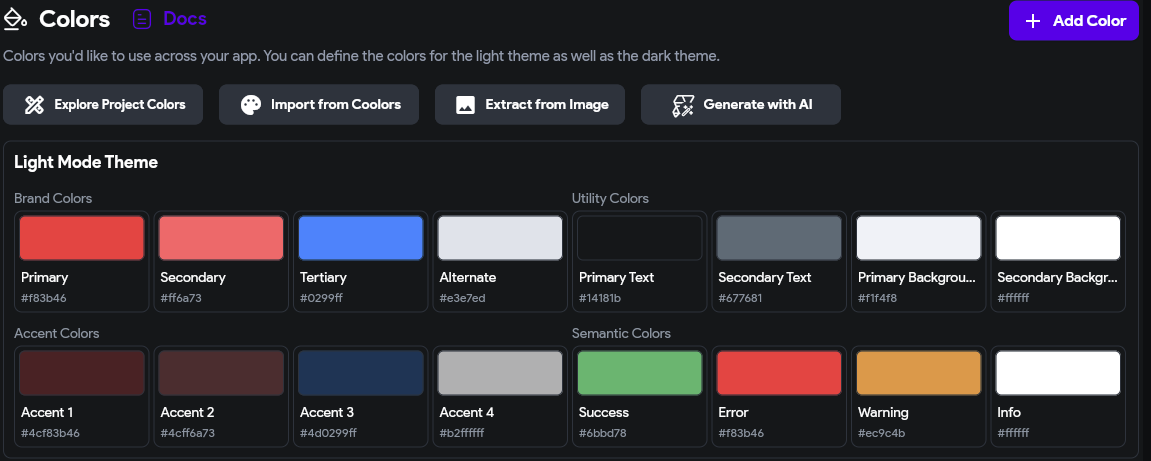
\includegraphics[width=1\linewidth]{images/Screenshot 2024-01-27 at 15.38.16.png}
    \caption{Ausschnitt der Theme Settings von FlutterFlow}
    \label{fig:flutterflow_themes}
\end{figure}

FlutterFlow bietet verschiedene Theme Settings. Dazu gehört die Farbeinstellung. Abbildung \ref{fig:flutterflow_themes} zeigt einen Ausschnitt davon. Das \textit{Light Mode Theme} beschreibt die als Standard verwendete Farbauswahl der App. Es gibt zudem ein alternatives \textit{Dark Mode Theme}, welches von Apps verwendet wird, wenn der User entsprechende Einstellungen im Betriebssystem oder in der App vorgenommen hat. Der Dark Mode bietet meist eine alternative Darstellung von User Interfaces, die deutlich dunkler als die Standardversion ist oder einen dunklen Hintergrund mit heller Schrift nutzt. 

Die Themes bestehen jeweils aus einer Vorauswahl von Farben, die jeweils nach ihrem Nutzungszweck benannt sind. Der primäre Farbton zum Beispiel wird im Verhältnis zu den darauf folgenden sekundären und tertiären Farbtönen am häufigsten in den Oberflächen der App vorkommen. \textit{Sematic Colors} werden in spezifischen Fällen angewandt, in denen Zustände mit Farben assoziiert werden, wie zum Beispiel rot im Fall eines Fehlers verwendet wird. 

Welche Farben genau verwendet werden sollen, lässt sich vom User mithilfe eines Farbauswahlwerkzeugs anpassen, es können auch Hash- oder RGB-Werte angegeben werden, die die gewünschten Farben beschreiben. 

Die gewählten Farben sind auf der \textit{Theme Settings}-Seite deutlich erkennbar, hierdurch lässt sich abschätzen, ob diese miteinander harmonieren oder nicht zusammenpassen.

\begin{verbatim}
class LightModeTheme extends FlutterFlowTheme {
  @Deprecated('Use primary instead')
  Color get primaryColor => primary;
  @Deprecated('Use secondary instead')
  Color get secondaryColor => secondary;
  @Deprecated('Use tertiary instead')
  Color get tertiaryColor => tertiary;

  late Color primary = const Color(0xFF4B39EF);
  late Color secondary = const Color(0xFF39D2C0);
  late Color tertiary = const Color(0xFFEE8B60);
  late Color alternate = const Color(0xFFE0E3E7);
  late Color primaryText = const Color(0xFF14181B);
  late Color secondaryText = const Color(0xFF57636C);
  late Color primaryBackground = const Color(0xFFF1F4F8);
  late Color secondaryBackground = const Color(0xFFFFFFFF);
  late Color accent1 = const Color(0x4C4B39EF);
  late Color accent2 = const Color(0x4D39D2C0);
  late Color accent3 = const Color(0x4DEE8B60);
  late Color accent4 = const Color(0xCCFFFFFF);
  late Color success = const Color(0xFF249689);
  late Color warning = const Color(0xFFF9CF58);
  late Color error = const Color(0xFFFF5963);
  late Color info = const Color(0xFFFFFFFF);
}
\end{verbatim}

Der vorangehende Quellcodeausschnitt stellt den zugehörigen, von FlutterFlow generierten Dart-Code dar. Für das \textit{Light Theme} wird eine Klasse definiert, die \textit{Color}-Datenfelder beinhaltet. Jedes dieser Felder steht für eine andere Farbe des Themes, zum Beispiel die Farbe \textit{primary}. Die Farben selbst sind als Hexadezimalzahlen definiert. Für Personen, die den Quellcode lesen, ist es schwer nachvollziehbar, um welche Farben es sich bei den Werten genau handelt.

\section{FlutterFlow - persönliche Einschätzung}

Nachdem einige Zeit mit der Plattform FlutterFlow an einem MVP für einen E-Shop gearbeitet wurde, sind die ein oder anderen Auffälligkeiten deutlich geworden. Diese Auffälligkeiten sind zum großen Teil auch persönliche Einschätzungen und sollen in den nachfolgenden Unterkapiteln aufgezeigt werden.
Außerdem sind alle in diesem Kapitel verwendeten Abbildungen Screenshots der FlutterFlow-Umgebung. Sie stammen aus der Zeit von Dezember 2023 bis Februar 2024.

\subsection{FlutterFlow}
FlutterFlow wurde im Zuge der Arbeit für das Testen einer Low-Code-Plattform verwendet und soll an dieser Stelle nur kurz erläutert werden.

FlutterFlow ist eine webbasierte, visuelle Entwicklungsplattform, die auf dem Flutter-Framework von Google basiert. FlutterFlow wurde von zwei ehemaligen Google-Ingenieuren gegründet. Es soll Designer:innen, Entwickler:innen und Unternehmen ganz allgemein das Erstellen mobiler Apps erleichtern.

Die Plattform bietet die Möglichkeit, Entwickler:innen, auch ohne tiefgreifende Programmierkenntnisse, plattformübergreifende mobile Anwendungen zu erstellen.
FlutterFlow integriert Backend-Funktionen. Das bedeutet, dass Entwickler:innen grundlegende Server- und Datenbankenfunktionalitäten ohne separate Backend-Entwicklung implementieren können. \cite{flutterflow_features}

\subsection{Visuelle Programmierung}
Die Plattform ist für den Einstieg in die Thematik (Web-)App-Programmierung sehr gut geeignet. Auch ohne Vorkenntnisse mit der Programmiersprache Dart, die FlutterFlow beziehungsweise Flutter verwendet, kann eine vollständig funktionsfähige Applikation entwickelt werden, ohne auch nur eine Zeile Quellcode je gesehen zu haben.

\subsection{Erste Erfolge}
Beim Arbeiten mit FlutterFlow wird sofort deutlich, dass man sehr schnell Ergebnisse sehen kann.
Die Entwicklungsumgebung hilft dem Entwickler beziehungsweise der Entwicklerin, die Rahmenbedingungen für das Projekt so schnell wie möglich abzunehmen, sodass sich darum nur ganz kurz gekümmert werden muss. Hierbei ist wichtig zu erwähnen, dass man sich darum kümmern muss. Es gibt keinen Weg daran vorbei, was gut ist, damit schon einige essenzielle Dinge ganz zu Beginn geklärt werden und in Zukunft beispielsweise beim Anpassen des Designs an zentralen Stellen die richtigen Änderungen gemacht werden können.

Es kann sich ganz unproblematisch dazwischen entschieden werden, ob die (Web-)Applikation vollständig nach den eigenen Wünschen umgesetzt oder ob eine Vorlage verwenden werden soll.
In Abbildung \ref{fig:startseite_projekterstellung} sieht man die Startseite bei der Erstellung eines Projekts in FlutterFlow.
\begin{figure}[h]
    \centering
    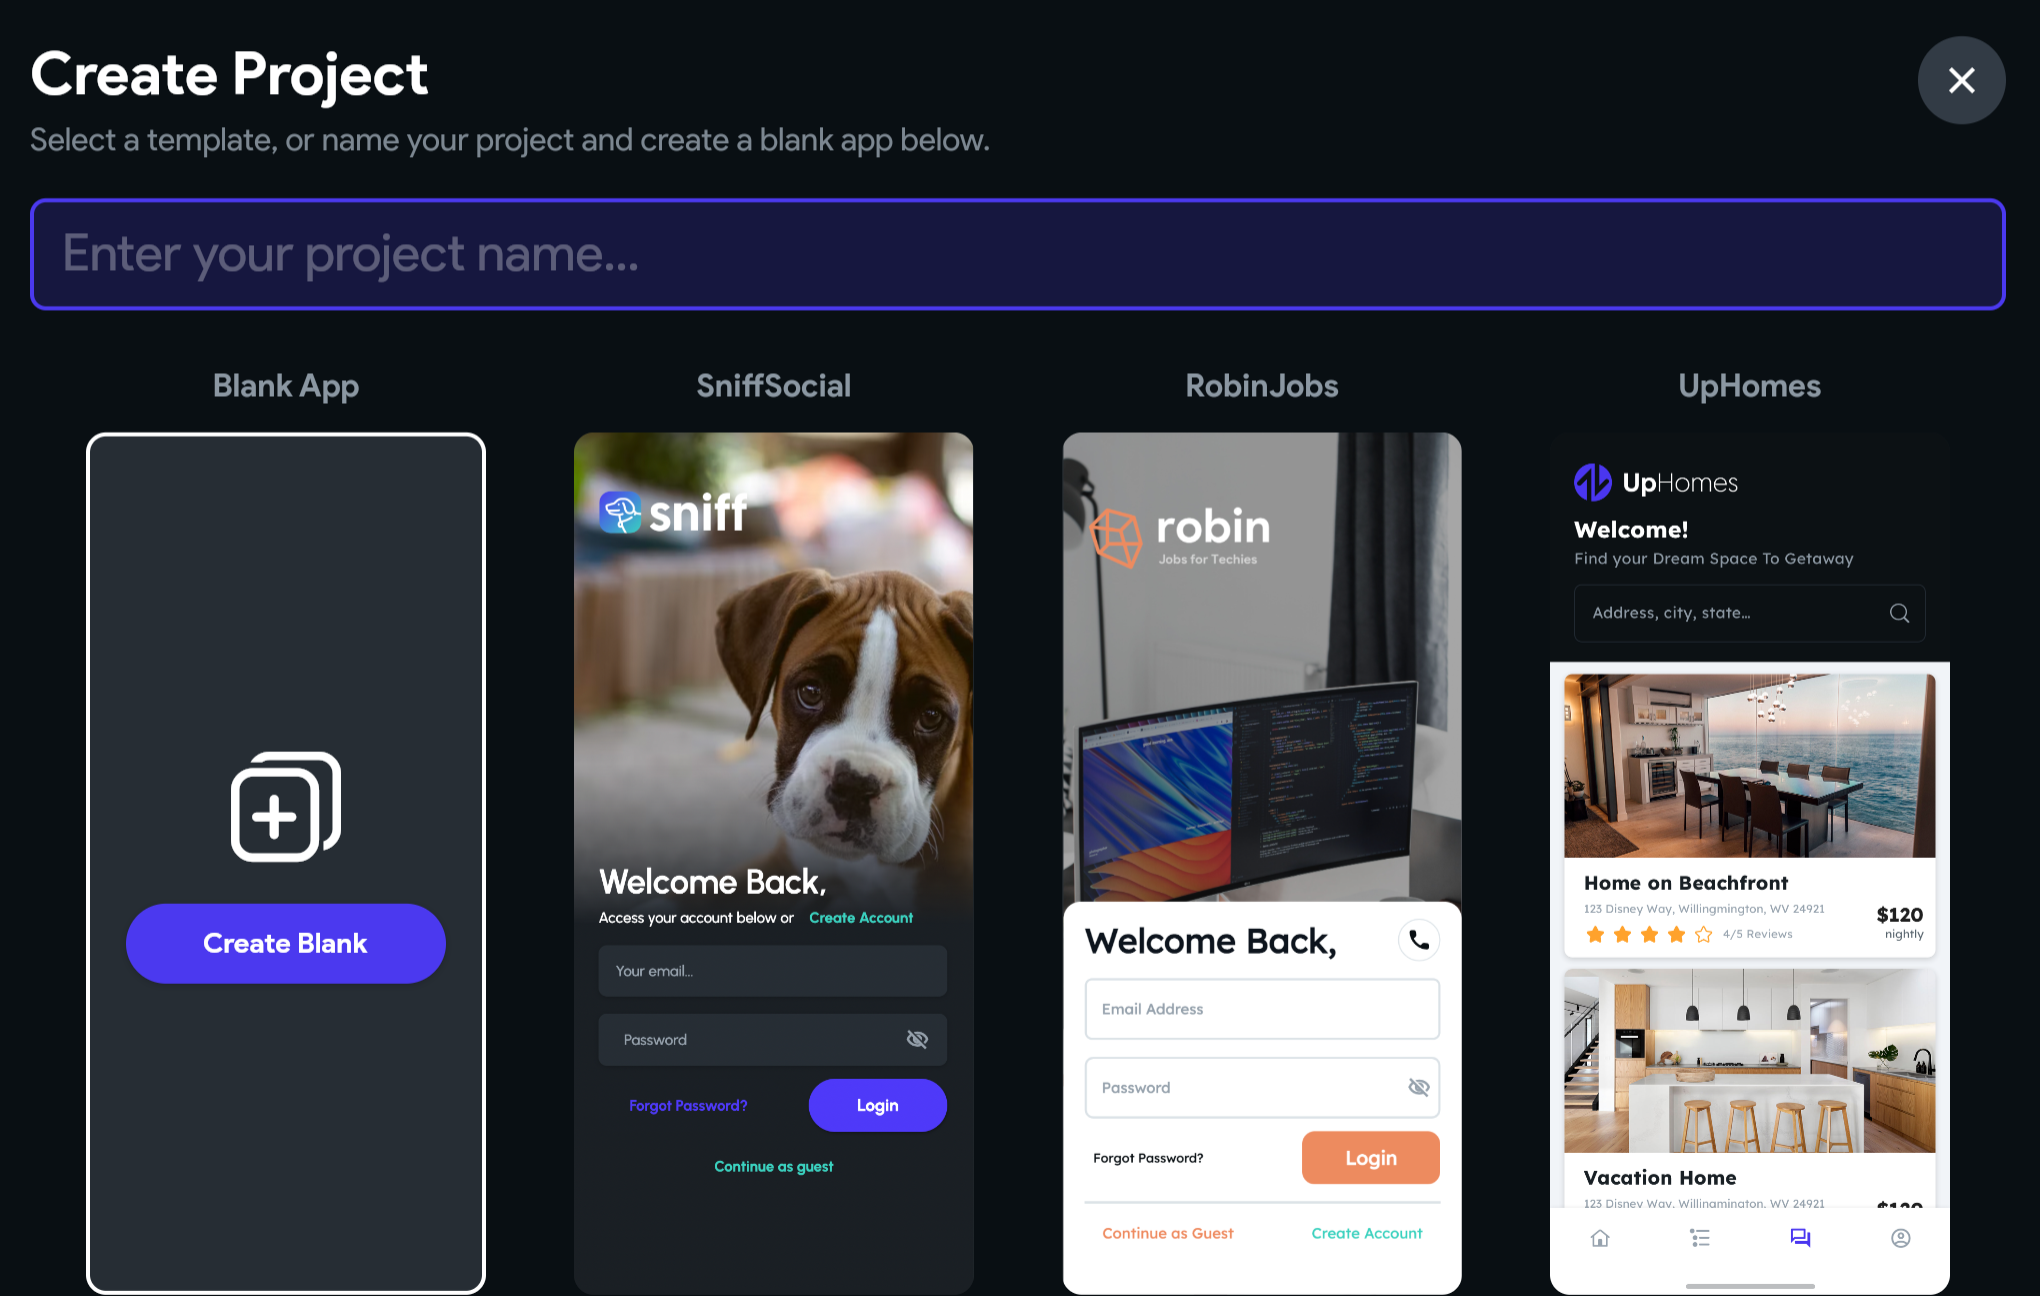
\includegraphics[width=1\linewidth]{images/FF_projekt_erstellen.png}
    \caption{Projekterstellung mit FlutterFlow}
    \label{fig:startseite_projekterstellung}
\end{figure}
Wurde sich nun entschieden und die ersten Seiten sind erstellt, können relativ zügig Elemente aus der \textit{Widget Palette} auf die gewünschte Seite an die gewünschte Stelle gezogen werden. Das ist in Abbildung \ref{fig:widget_palette} zu sehen.
\begin{figure}[h]
    \centering
    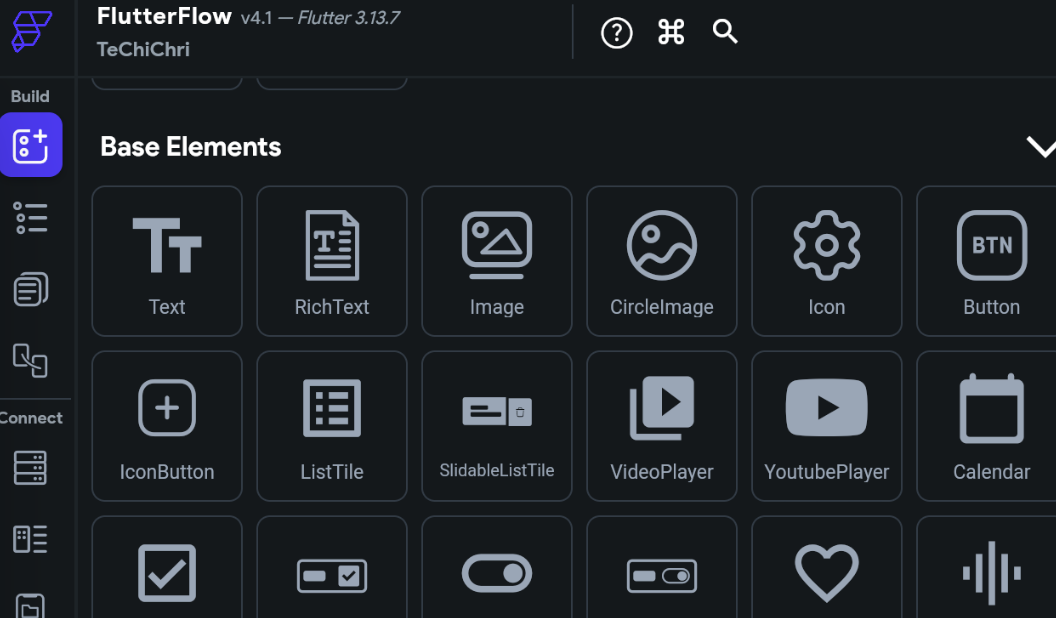
\includegraphics[width=1\linewidth]{images/FF_widget_palette.png}
    \caption{Widget Palette}
    \label{fig:widget_palette}
\end{figure}

\subsection{Hinweise}
Schnell wird deutlich, wenn man Fehler macht und beispielsweise ein Problem erzeugt, das die (Web-)App zum Absturz bringen würde, gibt die Plattform Hinweise diesbezüglich und verhindert den Vorgang. Das ist so üblich bei Low-Code-Plattformen. Es können auch keine Syntaxfehler entstehen.
Auch gibt die Plattform Hinweise darüber, wie die User Experience optimiert werden könnte, beispielsweise durch Vorgaben zum Format. Dies kann man in der Abbildung \ref{fig:optimization_ff} betrachten.
\begin{figure}[h]
    \centering
    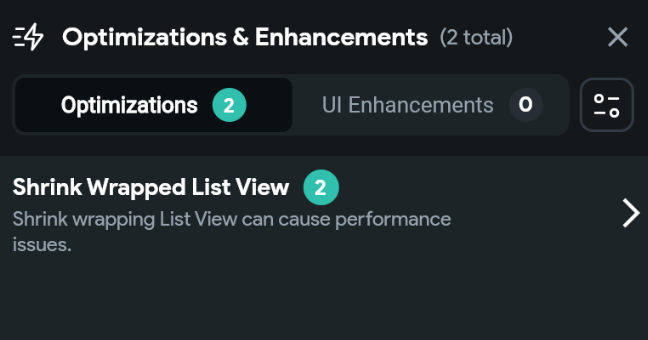
\includegraphics[width=1\linewidth]{images/FF_optimization.png}
    \caption{Optimization \& Enhancement}
    \label{fig:optimization_ff}
\end{figure}

\subsection{Eingeschränkte Anpassungsmöglichkeiten}
Bei der Arbeit am MVP für den E-Shop sind keine Einschränkungen aufgetaucht, weil es sich hierbei nur um eine sehr heruntergebrochene Version der Applikation handelt. Es sei jedoch nicht aus den Augen zu verlieren, dass No-Code beziehungsweise Low-Code-Plattformen bestimmte Vorgaben, Vorlagen und Widgets haben, die zwar abgeändert werden können, wenn es aber darauf ankommt, eine hochgradig spezifische und angepasste Funktion oder Design zu implementieren, es zu Problemen kommen kann. Das liegt daran, dass nur begrenzt Kontrolle über den Quellcode besteht, da dieser zum großen Teil automatisch generiert wird.

An einer Stelle sollte eine Anpassung vorgenommen werden, die ein gewisses Verständnis des Quellcodes mit sich bringt.
Im Warenkorb sollte eine Funktion geschrieben werden, die die Summe des Gesamtbetrags abändert, wenn man ein Produkt aus dem Warenkorb entfernt. Dafür wurde auf die Variable \textit{price} aus dem Dokument \textit{product} und auf den App State \textit{cartSum}. An dieser Stelle musste eine \textit{Code Expression} hinzugefügt werden, da es bei FlutterFlow bei der \textit{Increment/Decrement}-Funktion keine Möglichkeit gibt, eine Variable von einer anderen Variable abzuziehen. Das Ganze sieht man dann in Abbildung \ref{fig:decrement_fct}.
\begin{figure}[h]
    \centering
    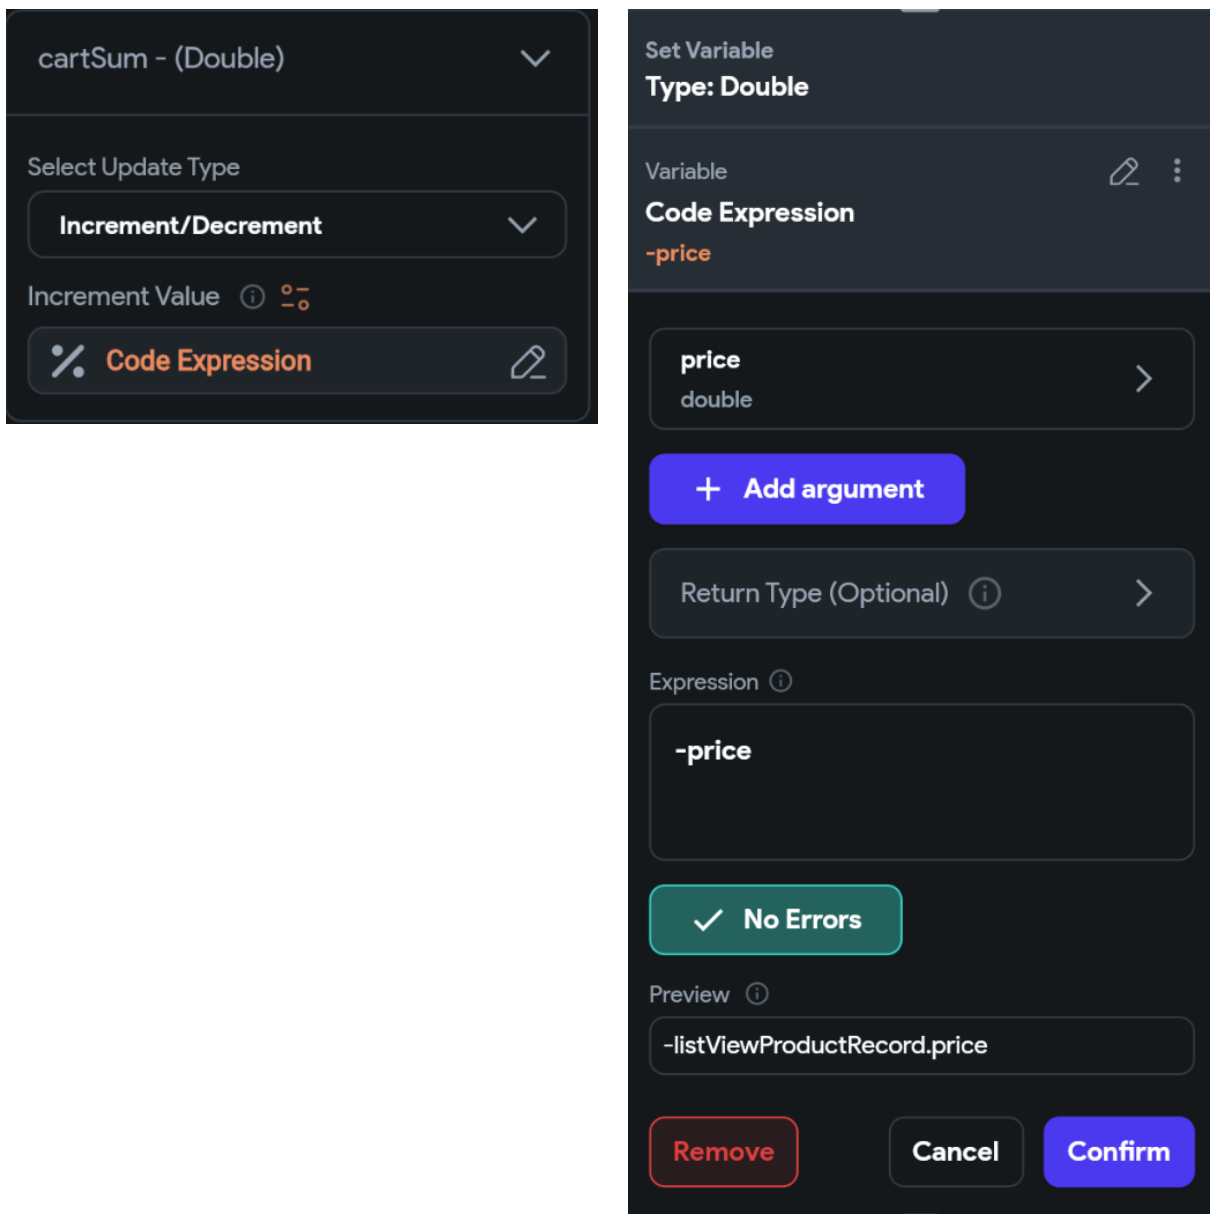
\includegraphics[width=1\linewidth]{images/FF_decrement.png}
    \caption{Warenkorb: Decrement-Funktion}
    \label{fig:decrement_fct}
\end{figure}
\subsection{Community und Support}
Beim Arbeiten mit FlutterFlow und der Fehlerbehebung fällt auf, dass triviale Probleme durch Forendiskussionen der Community sowie Dokumentationen von Flutter selbst relativ schnell gelöst werden können. Hierbei wird vor allem auf die \textit{FlutterFlow Introduction} \cite{flutterflow_doc}verwiesen, die eine Schritt-für-Schritt-Anleitung bietet, um ein erstes eigenes Projekt umzusetzen.

Außerdem bietet der YouTube-Kanal von FlutterFlow eine große Anzahl an Tutorials. Dort werden unter anderem auch ganze Livestreams zur Verfügung gestellt, um bei größeren Projekten mitzuarbeiten. Ein Beispiel: \cite{flutterflow_youtube}


\section{Ausblick und Zukunft}

Im Abschnitt \ref{sec:Aktuelle_Nutzung} zeigt Abbildung \ref{fig:lowcode_nutzer}, dass die Hälfte aller befragten Unternehmen mit mehr als 1000 Beschäftigten angeben, Software mit Hilfe von Low-Code-Plattformen entwickeln. Dies entspricht in etwa dem Anteil derer, die angeben, ausschließlich mit High-Code zu entwickeln.  

Ob und in welcher Form Low-Code-Entwicklung in den nächsten Jahren weiterverwendet wird, ist nur schwer voraussehbar.

Einerseits bietet die aktuelle Entwicklung von Künstlicher Intelligenz einen neuen Ansatz in Bezug auf Low-Code, andererseits gibt es auch Bedenken bezüglich Sicherheitslücken von Low-Code-Plattformen. \cite{studie_low_code}

\section{Zusammenfassung}
In dieser Arbeit wurde das Softwareentwicklungsprinzip Low-Code im Kontext vergangener und aktueller Entwicklungen vorgestellt. Dabei wurde festgestellt, dass einige der Ansätze daraus bereits vor Jahrzehnten Anwendung fanden, wenn auch nur in begrenztem Umfang. Es wurde überlegt, welche Szenarien in großen Entwicklungsteams auftreten und wie sie mit dem Einsatz von Low-Code bewältigt werden können. Ferner wurde untersucht, welche Gründe für die aktuelle Beliebtheit von Low-Code/No-Code-Plattformen sprechen. Als mögliches Risiko bei der Nutzung von Low-Code-Plattformen wurde die Abhängigkeit vom jeweiligen Anbieter identifiziert. Anhand eines Beispielprojekts wurde die Arbeit mit einer Low-Code-Plattform veranschaulicht. Als Ergebnis dieses Experiments konnte festgestellt werden, dass die Entwicklung eines simplen MVP ohne technisches Know-how durchgeführt werden konnte, was dem Versprechen der Low-Code-Anbietern entspricht. Wenn es aber darum geht, eine komplexere Anwendung zu entwickeln, so ist es früher oder später vonnöten, den Quellcode manuell anzupassen, um die uneingeschränkte Kontrolle behalten zu können.

%% The next two lines define the bibliography style to be used, and
%% the bibliography file.
\bibliographystyle{ACM-Reference-Format}
\bibliography{quellen}


%% If your work has an appendix, this is the place to put it.
\appendix

\section{Anhang}

\subsection{Übungsaufgaben}
\subsubsection{Aufgabe 1}
Anwenden von FlutterFlow.
Erstellen Sie sich einen FlutterFlow-Account. Dieser ist für Studierende kostenlos. Öffnen Sie folgende URL um das genannte Projekt zu öffnen: \href{https://app.flutterflow.io/project/te-chi-chri-9rmiar?tab=uiBuilder&page=products}{FlutterFlow Projekt}.
Den dazugehörigen generierten Quellcode finden Sie in folgendem Git Repository: \href{https://github.com/Beleg-12-Low-Code-Ansatze/abgabe}{Flutter Sourcecode}

Alternativ können Sie ein eigenständiges FlutterFlow Projekt anlegen, oder eines der vorhandenen Beispielprojekte verwenden. Verknüpfen Sie das Projekt mit einem Github Account, eine Anleitung hierzu finden Sie im Developer Menu Ihres FlutterFlow Projektes. 
Suchen Sie nun im Quellcode nach verschiedenen Komponenten des Projektes.

\subsubsection{Aufgabe 2}
Ändern Sie in diesem Projekt den App-Namen und nehmen Sie generelle Design-Änderungen vor.

\subsubsection{Aufgabe 3}
Entwickeln Sie eine minimalistische To-Do-Liste mit der Hilfe von FutterFlow. Die App sollte grundlegende Funktionen zum Hinzufügen, Anzeigen und Löschen von Aufgaben bieten.
Gehen Sie dabei auf folgenden Aspekte ein:
\begin{enumerate}
    \item Benutzeroberfläche
    \item Funktionalität
    \item Datenbankintegration
\end{enumerate}

\end{document}
\endinput
%%
%% End of file `sample-acmtog.tex'.
